\documentclass[a4paper,11pt]{report}

\usepackage[a4paper,left=3cm,right=3cm,top=2.5cm,bottom=2.5cm,includeheadfoot]{geometry}
\usepackage[utf8]{inputenc}
\usepackage[english]{babel}
\usepackage{fancyhdr}
\usepackage{amsmath}
\usepackage{amssymb}
\usepackage{bm}
\usepackage[noabbrev,capitalise]{cleveref}
\usepackage[square]{natbib}
\usepackage{url}
\usepackage{graphicx}
\usepackage{listings}
\usepackage{chngcntr}
\usepackage{graphicx}
\usepackage{color}
\usepackage{float}

%REMOVE - DARK MODE
%\usepackage{xcolor}
%\pagecolor[rgb]{0,0,0} %black
%\color[rgb]{0.5,0.5,0.5} %grey 

\fancyhf{}
\chead{\leftmark}
\cfoot{\thepage}
\setlength{\headheight}{14pt}
\renewcommand{\headrulewidth}{0.5pt}
\newcommand{\HRule}[1]{\rule{\linewidth}{#1}}

\counterwithout{figure}{chapter}
\counterwithout{table}{chapter}
\counterwithout{equation}{chapter}

\begin{document}

%title page
\title{ 
    \vspace{-4cm}
    \begin{figure}[h]
    \centering
    \includegraphics[width=0.3\textwidth]{figures/ub_logo.png}
    \end{figure}
    \vspace{1cm}
	\HRule{2pt}\\
	\LARGE \textbf{Exploring the Capabilities of Automatic 3D Model Generation: A Comparative Study}\\
	\HRule{2pt}\\
	\vspace{2cm}
	\normalsize Bachelor's Thesis\\
	\vspace{0.5cm}
	in the applied computer science course of the faculty of business informatics and applied computer science at the Otto-Friedrich-University of Bamberg\\
	\vspace{0.5cm}
	Faculty of Computer Graphics\\
	\vspace{4cm} %4cm is normal, change if title is fixed
}

\date{}

\author{
    \begin{minipage}{\textwidth}
    \begin{flushleft}
    Author: Andreas Franz \textsc{Schwab}\\
    \vspace{0.5cm}
    Examiner: Prof. Dr. Sophie \textsc{Jörg}
    \end{flushleft}
    \end{minipage}
}

\maketitle
\begin{abstract}

The exploration of automatic 3D model generation represents a significant stride in the realm of computer vision and machine learning. This thesis delves into the capabilities of this innovative technology, focusing on a comparative study of various methodologies that facilitate the creation of 3D models from textual and image inputs. The importance of this topic stems from the increasing demand for efficient and accurate 3D model generation in various applications, ranging from virtual reality and gaming to medical imaging.

Despite the advancements in this field, there exists a research gap in comprehensively understanding and comparing different automatic 3D model generation techniques, particularly in the context of their effectiveness, accuracy, and applicability. This thesis aims to bridge this gap by conducting a thorough analysis of selected methods, including DreamFusion \citep{pooleDreamfusion}, Magic3D \citep{lin2023magic3d}, and Fantasia3D \citep{chen2023fantasia3d} for text input, and Magic123 \citep{qian2023magic123} and Wonder3D \citep{long2023wonder3d} for image input. The research methods include a detailed experimental setup that uses both subjective evaluations and performance metrics to analyze these technologies.
    
The key message of this thesis highlights the differentiated capabilities and limitations of the individual methods and provides insights into their applicability and potential for future development. The results show significant differences in the accuracy and efficiency of the methods examined and highlight the strengths and weaknesses of the individual techniques in different scenarios.
    
By offering a comprehensive comparison of various methodologies in automatic 3D model generation, this thesis not only aids in the understanding of these technologies but also paves the way for future research, particularly in addressing generative biases and exploring emerging trends.

\end{abstract} 


%toc
\pagenumbering{Roman}
\setcounter{page}{3}
\setcounter{tocdepth}{2}
\tableofcontents


%tables, figures
\listoftables
\listoffigures
\newpage

%content
\pagestyle{fancy}
\pagenumbering{arabic}
\setcounter{page}{1}

\chapter{Introduction}~\label{ch:introduction}

In today's rapidly evolving digital landscape, the demand for 3D models continues to grow, driven by the ever-increasing need for immersive and realistic visual experiences. Generative AI techniques have proven to be a transformative force, enabling researchers and practitioners to develop innovative methods that automate the complicated process of creating 3D models. These groundbreaking innovations have the potential to reshape our digital interactions by enabling advanced simulations, in-depth analysis and captivating visualizations of complex real-world phenomena.

Starting out in 3D synthesis can be a challenging experience, particularly for novices with limited prior knowledge. While directly applying the models outlined in Chapter~\ref{ch:models} may appear straightforward, acquiring a more in-depth understanding of the diverse methodologies and their foundational principles greatly enriches the learning process. This deeper understanding not only improves the practical application of these models, but also opens the door to future advances in the field of automatic 3D model generation.

This thesis provides a comprehensive examination into a variety of models and technologies in automated 3D model generation, offering a detailed analysis of their mechanisms, capabilities, and limitations. The study focuses on evaluating the technologies' effectiveness, emphasizing their proficiency in creating functionally robust and aesthetically appealing 3D models. This research contributes to the fields of computer graphics and artificial intelligence, serving as a valuable resource for novices in automatic 3D model generation and inspiring future researchers.

To provide a foundation for this exploration, a comprehensive examination of the fundamentals of 2D generative AI is undertaken. This includes a comprehensive understanding of key generative models such as Variational Autoencoders (VAEs) \citep{kingmaVAE,rezendeVAE}, Generative Adversarial Networks (GANs) \citep{goodfellowGAN} and Diffusion Models \citep{yangdiffusionSummary,hoDDPMs, sohlDDPM}. Additionally, a brief introduction to Contrastive Language-Image Pre-training (CLIP) \citep{radfordCLIP} and Multilayer Perceptron (MLP) is given. The section concludes with an overview of various forms of 3D representation, including Meshes, Point-clouds, Voxels, Neural Radiance Fields (NeRFs) \citep{mildenhallNERF}, Deep Marching Tetrahedra (DMTets) \citep{shen2021DMTet}, and Instant Neural Graphics Primitives (InstantNGPs) \citep{M_ller_2022}.

This research further evaluates various approaches to generating 3D models based on both images and text input. The methods examined include DreamFusion \citep{pooleDreamfusion}, Magic3D \citep{lin2023magic3d}, Fantasia3D \citep{chen2023fantasia3d}, Magic123 \citep{qian2023magic123} and Wonder3D \citep{long2023wonder3d}. Each method presents unique challenges and opportunities, and their results are thoroughly examined through a comparative study. 

The evaluation involves the application of rigorous performance evaluation metrics covering a spectrum of critical aspects. These metrics include the accuracy of the input and results to ensure that the generated models accurately match the input and maintain the intended properties. In addition, the level of detail of these models is examined to assess their ability to capture complicated features and nuances. An important criterion is realism, i.e.~the ability of the generated models to reflect the authenticity of their real-life counterparts. Furthermore, technical aspects such as symmetry and model integrity are also examined to check the structural soundness and coherence of the generated 3D models. This comprehensive analysis leads to an in-depth understanding of the strengths and weaknesses of the individual methods investigated.

In addition, this thesis casts a discerning eye towards the evolving landscape of 3D modeling and highlights emerging trends that have the potential to reshape the field. These trends include innovations such as video-to-3D methods that open up new dimensions in the creation of three-dimensional scenes. In addition, the important topic of inherited biases is discussed, highlighting the need for more in-depth research to ensure the fairness of these methods. By exploring these unexplored areas, the aim is to promote a fairer and more progressive future for the field of 3D modeling.
\chapter{Basics}
\label{ch:basics}

The chapter provides the groundwork necessary for the comparative analysis of automatic 3D model generation techniques by introducing the key technologies that drive these methods. It is essential to have a common understanding of the generative machine learning algorithms and 3D data representations that form the basis of this field.

The section starts with Variational Autoencoders (VAEs) \citep{kingmaVAE,rezendeVAE}, which serve as probabilistic frameworks for learning complex data representations. Generative Adversarial Networks (GANs) \citep{goodfellowGAN} are then discussed, highlighting their unique training dynamics that include both generator and discriminator components. The section further explores the domain of Diffusion Models, particularly Denoising Diffusion Probabilistic Models (DDPMs) \citep{hoDDPMs,sohlDDPM}, while also briefly covering Stochastic Gradient Methods (SGMs) \citep{song2019SGM} and Stochastic Differential Equations (SDEs) \citep{song2020score,song2021maximum}. These mentioned models, as captured by the "generative learning trilemma" \citep{xiao2022tackling}, highlight the balance and compromises inherent in their design and application.

\begin{figure}[ht]
    \centering
      \includegraphics[width=.4\columnwidth]{figures/BasicTrilemma.png}
      \caption{A short characterization of the most important features and drawbacks of the generative models discussed in this section.~\citep{xiao2022tackling}}
      \label{fig:generativeTrilemma}
\end{figure}

The chapter also examines Contrastive Language-Image Pre-training (CLIP) \citep{radfordCLIP}, showcasing its ability to bridge natural language and visual data, thereby facilitating text-guided 3D model generation. Lastly, various forms of representation of 3D data are examined, including Meshes, Point-Clouds, and Voxels, constituting the foundational structure of 3D objects in computational environments. Proficiency in these representations is required for comprehending the 3D model generation.

//TODO check Final Diffusion Model

\section{Variational Autoencoders - VAEs}
\label{VAEs}

Based on the seminal work by \citeauthor{diggleImplicitPrescribed}, generative models can be classified into two broad categories. Prescribed models employ a well-defined, often parametric, mathematical expression for the probability density function (pdf), which enables easier analytical interpretation of the distributions. In contrast, implicit models synthesize new data samples without relying on an explicit pdf, approximating the underlying data distribution on which they were trained \citep{diggleImplicitPrescribed}. Variational Autoencoders (VAEs), which inherit the foundational architecture of autoencoders, belong to the prescribed models category as they require an explicit formulation of the probability density function (pdf) to function effectively. This feature makes VAEs suitable for tasks that require not only the generation but also the understanding of complex data distributions. \citep{kingmaVAE,rezendeVAE,GoodfellowDeepLearning}. Generative Adversarial Networks (GANs) \citep{goodfellowGAN}, discussed later, are a prime example ofthe latter category.

VAEs are essentially based on the architecture of autoencoders, which consist of an encoder and a decoder. The encoder aims to transform the input data into a low-dimensional latent space representation, commonly referred to as a "code" or "bottleneck" \citep{hintonCode, GoodfellowDeepLearning}. This code captures the most relevant features of the input while reducing its dimensionality. Then, the decoder attempts to reconstruct the original input from the obtained latent vector using a loss function. As explained by Goodfellow et al, an autoencoder that only succeeds in copying the exact representation of the input data does not itself prove useful. The essence of autoencoders lies in their ability to copy approximately rather than perfectly, which forces the model to prioritize which aspects of the input to copy \citep{GoodfellowDeepLearning}. This strategic approach often directs autoencoders to "learns useful properties of the data" \citep{GoodfellowDeepLearning}. To summarize, he main goal of an autoencoder is not the reconstruction itself, but the extraction of a meaningful latent vector that serves as a simplified representation of the input data.

The ability to reduce dimensionality has practical implications for improving the efficiency of classification tasks by reducing computational and memory overhead \citep{GoodfellowDeepLearning}. When paired with information retrieval, this dimensionality reduction makes searching in certain low-dimensional spaces particularly efficient \citep{GoodfellowDeepLearning}. Despite these advantages, traditional autoencoders are not designed to generate new data; their main function is to copy and reconstruct the given input \citep{GoodfellowDeepLearning}.

\begin{figure}[ht]
    \centering
      \hspace{.8cm}
      \includegraphics[width=.7\columnwidth]{figures/Autoencoder.png}
      \caption{Autoencoder: The encoder reduces the input dimension to a latent vector that captures the most important features. The decoder then uses this vector to reconstruct the input, with training aimed at minimizing reconstruction loss.}
      \label{fig:figureAE}
    \end{figure}


In variational autoencoders (VAEs), the encoder compresses the input into a space of latent variables and forms a probability distribution over these latent variables called \( q(z|x) \). This distribution helps with robustness against overfitting and enables the model to synthesize new analog data points. During the training phase, VAEs recognize specific regions in the latent variable space, similar to "pools," for different categories of data, allowing for a structured approach to data representation. Unlike standard autoencoders, where it is unclear where a useful latent vector can be sampled for the decoder, VAEs overcome this problem by restricting the latent space to known regions from which vectors can be safely sampled, as cited in \citep{doerschVAE}.

The procedure begins by selecting a sample \( z \) from a code distribution defined by the model, denoted \( p_{model}(z) \). This sample \( z \) is then passed through a differentiable generator network \( g(z) \). A sample \( x \) is then drawn from the distribution \( p_{model}(x; g(z)) \), where its properties are shaped by the processed \( z \) \citep{GoodfellowDeepLearning}. During the training phase, an approximate inference network, also called an encoder \( q(z|x) \), is used to infer \( z \) from \( x \), while \( p_{model}(x|z) \) works as a decoder network to reconstruct \( x \) from \( z \) \citep{GoodfellowDeepLearning}. The main training objective is embodied in the formula:
        
\begin{align}
  L(q) &= \mathbb{E}_{z \sim q(z|x)} \log p_{model}(z, x) + H(q(z|x)) \\
  &= \mathbb{E}_{z \sim q(z|x)} \log p_{model}(x|z) - D_{KL}(q(z|x) || p_{model}(z)) \\
  &\leq \log p_{model}(x)
\end{align}
        
Here, \( L(q) \) acts as a scorecard to evaluate the performance of UAE. The first term \( \log p_{\text{model}}(x|z) \) evaluates how well the UAE can fill in the details to recover the original input, while the second term \( D_{\text{KL}}(q(z|x) || p_{\text{model}}(z)) \) evaluates the complexity of the VAE representation compared to the original term, aiming for simplicity, as mentioned in \citep{GoodfellowDeepLearning}. 
        
The decoder in VAEs either reconstructs the original input or synthesizes new outputs from sampled latent variables. This process is optimized by a loss function that includes both the reconstruction loss and a regularization term based on the Kullback-Leibler (KL) divergence \( D_{\text{KL}} \). This divergence measures the discrepancies between the estimated and true data distributions \citep{kingmaVAE} and improves the model's ability to effectively generalize to unseen data.
        
Through this mechanism, VAEs continuously refine their representation and reconstruction process, improving the generation of new data points that resemble the original training data while maintaining a simplified and structured latent space.

\begin{figure}[ht]
    \centering
      \hspace{.8cm}
      \includegraphics[width=.9\columnwidth]{figures/VAE.png}
      \caption{Functionality of a Variational Autoencoder, demonstrating incorporation of the latent distribution - the mean and standard deviation - for enhancing generative capabilities.}
      \label{fig:figureVAE}
\end{figure}

Despite their capabilities, VAEs exhibit some limitations. According to \citeauthor{GoodfellowDeepLearning}, the generated samples can often be blurry. The reason for this is not fully 
understood, but the blurriness observed may be due to their optimization process, which minimizes Kullback-Leibler divergence. This could lead the model to assign high probabilities to "points that occur in the training set, but may also assign high probability to other points [...] which may include blurry images" \citep{GoodfellowDeepLearning}. The Gaussian distribution often used in VAEs for the generative model may also contribute to this effect, as it can ignore minor features in the input data \citep{GoodfellowDeepLearning}. Another issue is that VAEs typically utilize only a small portion of the latent space, which might further compromise the quality of generated images \citep{GoodfellowDeepLearning}. The performance of the model is also sensitive to the choice of priors for the latent space, making hyperparameter tuning an essential aspect of working with VAEs \citep{kingmaVAE, higginsVAE}. 


\section{Generative Adversarial Networks - GANs}
\label{GAN}

There are two main approaches in Machine learning methods, 
supervised learning and unsupervised learning. Supervised learning requires extensive control and a vast amount of labeled data sets, whereas unsupervised learning offers a more straightforward approach by not requiring classified data to learn a model.

In supervised learning, the ML algorithm learns from a labeled data set where each data point is related to a corresponding target or output value. This enables the algorithm to make predictions or classify new, unseen data based on the patterns it has learned from the labeled examples. The model's predictive capabilities are continuously refined by comparing its outputs to the expected outputs from the training dataset. Through this iterative process, adjustments can be made to enhance the model's performance and generate improved outputs. Yet, it is quite expensive and time-consuming to obtain the large amount of required data as it is often labeled manually by human experts. On the other hand, with the use of generative modeling, Unsupervised learning aims to discover patterns or structures within some unlabeled data. It demonstrates to be particularly useful when labeled data is scarce or unavailable. This concept of unsupervised learning sets the stage for understanding how implicit generative models like GANs address a significant limitation and offer a distinct advantage.

"When a deep neural network is used to generate data, the corresponding density function may be computationally intractable" \citep{goodfellowGAN}. Unlike traditional generative models, implicit generative models do not require the explicit design of a density function to describe the patterns in the data. Instead, they use a sample generation process that produces new samples resembling the existing ones \citep{goodfellowGAN}. Before Generative Adversarial Networks were introduced, the leading implicit generative model was the generative stochastic network, "which is capable of approximately generating samples via an incremental process based on Markov chains" \citep{goodfellowGAN}. Markov chains are a way of describing a sequence of events or states, where probability of transition to the succeeding state is solely dependent on current states. This approach, however,  can be time-intensive and may not always yield accurate results. GANs, on the other hand, directly generate high-quality samples in a single step, overcoming the limitations of incremental generation methods. It is useful to point out that the numerous steps of GAN training refer to iterative updating of model parameters rather than incremental sample generation.

The adversarial aspect of GANs arises from the game-like competition between two neural networks: the generator and the discriminator. The generator is responsible for creating fake inputs or samples, which are then passed to the discriminator. The discriminator's role is to differentiate between real samples from the domain set and the fake samples generated by the generator.

\begin{figure}[ht]
\centering
  \includegraphics[width=1\columnwidth]{figures/Generator.png}
  \caption{Simplified functionality of a Generative Adversarial Network}
  \label{fig:figureGAN}
\end{figure}

Initially, the discriminator is trained on a dataset of unlabeled data, aiming to learn the characteristics and attributes of the desired output. Once it becomes proficient at identifying the genuine objects, it is presented with examples of non-objects and its ability to distinguish these examples is assessed. 
Subsequently, the generator utilizes random input vectors to generate counterfeit versions of the desired objects. 
The discriminator then assesses the authenticity of these outputs and shares the result. Based on this feedback, the generator or the discriminator adjust their behavior. This iterative process, facilitated by an iterator, involves creating samples, updating the models, and repeating the cycle. Gradually, the generator becomes highly skilled at producing realistic outputs that the discriminator can no longer distinguish from real ones. This process is referred to as a zero-sum game, where there is always a winner and a loser. The winner remains unchanged, while the loser updates its model based on the feedback received from the discriminator.

For Images, the Discriminator and the Generator are often implemented as Convolutional Neural Networks (CNNs), which excel at recognizing patterns in images and are commonly used for object identification.
GANs are not limited to images, they can also be applied to tasks such as video frame prediction, image enhancement to improve image quality, and encryption \citep{goodfellowGAN}.

GANs pose a substantial challenge in their training process as they are hard to train \citep{goodfellowGAN}. In addition, \citeauthor{brophyGAN} highlight three important problems commonly associated with GANs, among others. These issues, namely non-convergence, diminishing or vanishing gradients, and mode collapse, contribute to the inherent instability experienced during GAN training. Non-convergence refers to the failure of a GAN model to stabilize and reach a state of equilibrium. Instead, it continuously oscillates and fails to converge to a satisfactory solution. As a result, the model does not learn the underlying patterns of the data and can even diverge, leading to poor performance \citeauthor{brophyGAN}. Diminishing or vanishing gradients occur when the gradients used to update the generator become extremely small or even vanish altogether. This phenomenon is often caused by an overly successful discriminator that becomes too adept at distinguishing real and fake samples. As a result, the generator struggles to learn from the feedback provided by the discriminator, impeding its ability to generate high-quality samples \citeauthor{brophyGAN}. Mode collapse happens when the generator collapses, meaning it focuses on producing only a limited set of samples or outputs, typically lacking diversity and variety \citep{salimansNIPS}. In such cases, the generator fails to capture the full range of patterns and characteristics present in the training data, resulting in uniform and repetitive samples that do not adequately represent the true distribution \citeauthor{brophyGAN}.

\section{Diffusion models}\label{diffusion Models}

The limitations of VAEs and GANs, which were just stated above, have led to the emergence of diffusion models, a method that offer distinct advantages over traditional generative models. Diffusion models operate by progressively perturbing data with noise and then learning to reverse this process to generate new samples. 

~\cite{yangdiffusionSummary} distingueshe between three main approaches that dominate the study of diffusion models, which are going to be discussed shortly: Denoising Diffusion Probabilistic Models (DDPMs) \citep{hoDDPMs,sohlDDPM}, Score-based Generative Models (SGMs) \citep{song2019SGM}, and Stochastic Differential Equations (Score SDEs) \citep{song2020score, song2021maximum}.

\subsection{Denoising Diffusion Probabilistic Models}
DDPMs employ two Markov chains, a forward chain and a reverse chain, also known as the forward and reverse diffusion processes, seen in Figure~\ref{fig:figureForwardProcess} and Figure~\ref{fig:figureReverseProcess} \citep{sohlDDPM}. 

The forward diffusion process is comparable to latent variable models, sharing some similarities with Variational Autoencoders (VAEs), as focus is lying on a latent feature space of the initial data distribution. They differ in the fact that the forward process in DDPMs ``is fixed to a Markov chain that gradually [over a span of T steps] adds Gaussian noise to the data according to a variance schedule \(\beta_1, \ldots, \beta_T \)''~\cite{hoDDPMs}. This iterative process continues to add noise ``until all structures are lost'' \citep{yangdiffusionSummary} resulting in an image of pure noise. The introduction of noise aims to gradually steer the data distribution towards a more manageable prior distribution \citep{yangdiffusionSummary, pooleDreamfusion}. Mathematically, the forward process can be described in two equations:

\[
q(x_t | x_{t-1}) = \mathcal{N}(x_t; \sqrt{1 - \beta_t}x_{t-1}, \beta_t I) \quad \text{where} \quad \sqrt{1 - \beta_t}x_{t-1} = \mu_t \quad \text{and} \quad \beta_t I = \Sigma_t
\] 

\citep{martinez2023understanding}. This describes the process of adding noise to transform a data point \( x_{t-1} \) into a new data point \( x_t \). This transformation is probabilistic and follows a Gaussian distribution \citep{sohlDDPM, hoDDPMs}. The mean value of this distribution is slightly adjusted compared to the previous data point by the factor \( \sqrt{1 - \beta_t} \), which essentially corresponds to the data point \( x_{t-1} \) with a certain noise reduction. The parameter \( \beta_t \) controls the amount of noise added, where a larger \( \beta_t \) means more noise \citep{kingma2023variationalDM}. The covariance matrix, denoted \( \beta_t I \), implies that each element of the data is independently modified with the same amount of noise, since \(I\) represents an identity matrix where all outer diagonal elements are zero \citep{croitoru2023diffusion}.

\[q(x_{1:T} | x_0) = \prod_{t=1}^T q(x_t | x_{t-1}) \] 

\citep{martinez2023understanding}. In the second equation, the focus is on the entire sequence of data points from the original \( x_0 \) to \( x_T \), including all intermediate points \citep{martinez2023understanding}. This expresses the idea that to understand the probability of the entire noisy trajectory, one can calculate the probability of each step from \( x_{t-1} \) to \( x_t \) and then multiply these probabilities together. This is due to the Markov property, which states that each step is only dependent on the immediately preceding step \citep{martinez2023understanding}. This enables a comprehensive view of the transition probabilities over the entire process of noise induction, step by step.

\begin{figure}[ht]
\centering
  \includegraphics[width=1\columnwidth]{figures/manta_DDMP3.png}
  \caption{Forward process adding noise to an image}\label{fig:figureForwardProcess}
\end{figure}

The reverse chain is trained to approximate the inverse of the forward process using a deep neural network parameterized with~\(\Theta\), effectively removing the noise added by the forward chain \citep{sohlDDPM, yangdiffusionSummary}. The function \( p_\theta(x_{t-1} | x_t) \) is a probability distribution that estimates how to reverse the diffusion process. Given a data point \( x_t \), it attempts to predict the previous data point \( x_{t-1} \) before noise was added. It is modeled as a normal distribution with a mean \( \mu_\theta(x_t, t) \) and covariance \( \Sigma_\theta(x_t, t) \), both of which are functions parameterized by \( \theta \) \citep{yangdiffusionSummary}.

\[
  p_\theta(x_{t-1} | x_t) = \mathcal{N}(x_{t-1}; \mu_\theta(x_t, t), \Sigma_\theta(x_t, t))
\] 

\[p_\theta(x_{0:T}) = p_\theta(x_{T}) \prod_{t=1}^T p_\theta(x_{t-1} | x_t) \]

\citep{martinez2023understanding}. The latter function \( p_\theta(x_{0:T}) \) represents the probability of the entire sequence of data points from \( x_0 \) through \( x_T \) under the reverse process modeled by the neural network. It starts with an estimate of the final data point \( p_\theta(x_{T}) \) and works backwards through the sequence, multiplying the conditional probabilities \( p_\theta(x_{t-1} | x_t) \) for each step \citep{hoDDPMs,martinez2023understanding}. This function essentially provides a framework for reconstructing the original data from the noisy data by successively removing noise at each step, based on the learned parameters \( \theta \) \citep{yangdiffusionSummary}.


\begin{figure}[ht]
  \centering
    \includegraphics[width=1\columnwidth]{figures/manta_DDMP3.png}
    \caption{Forward process adding noise to an image}\label{fig:figureReverseProcess}
\end{figure}


The incremental introduction of the forward and backward diffusion processes offers an advantage as ``estimating small perturbations is more tractable than explicitly describing the full distribution with a single, non-analytically-normalizable, potential function'' \citep{sohlDDPM}.
According to \citep{hoDDPMs}, the neural network in the reverse process can be trained to predict one of three possibilities: the mean value of the noise at each time step, the original image itself, or the noise of the image \citep{hoDDPMs}. As previously mentioned, the second approach is not as advantageous. Hence, the research focuses on the first and last possibilities, which are essentially identical but parameterized differently. Predicting the image noise allows for straightforward subtraction of the noise from the image, resulting in a less noisy version. By employing this method iteratively, it becomes possible to completely learn an image from noise.

Nevertheless, DDPMs also have their drawbacks with the most severe being the time requirement to generate new samples \citep{xiao2022tackling}. ``This is caused by the fact that a Markov process has to be simulated at each generation step, which greatly slows down the process'' \citep{martinez2023understanding}. 

\subsection{Score-Based Generative Models}

SGMs \citep{song2019SGM} take a unique approach to generative modeling by prioritizing the learning of a score function that plays a central role in guiding the generative process. This function aims to capture the Stein score \citep{steinScore}, which is essentially ``the gradient of the log-density function at the input data point'' \citep{song2019SGM}. The score can be viewed as a vector field that indicates the direction that increases the data density the most \citep{song2019SGM}. This reveals how slight adjustments within the data can affect the overall distribution, informing the model on how to proceed with sample generation in a way that matches the actual data structure.

To train a neural network for SGMs,~\cite{song2019SGM} employ two techniques, namely Score matching and Langevin dynamics \citep{hyvarinenScoreMatching}. 
Score matching allows to train a neural network, referred to as a score network \( s_\theta(x) \), to predict the gradient of the logarithm of the probability density of the data \( \nabla_x \log p_{\text{data}}(x) \) directly without the need to first construct a model that can estimate the probability density \( p_{\text{data}}(x) \) itself \citep{song2019SGM}. The aim of this process is to minimize the difference between the predictions of the score network and the true gradient of the log-likelihood, which under certain conditions ensures that the trained network approximates the true score ``almost surely'' \citep{song2019SGM}. The term \( \frac{1}{2} \|s_\theta(x)\|^2_2 \) is part of the objective function that needs to be minimized and is used to regularize the scores predicted by the neural network while the term \( tr(\nabla_x s_\theta(x)) \), involving the trace of the Jacobian \citep{song2019SGM} of the score function, further refines the objective function by capturing the divergence of the score vector field. 

\[
\mathbb{E}_{p_{\text{data}}(x)} \left[ \text{tr}(\nabla_x s_\theta(x)) + \frac{1}{2} \|s_\theta(x)\|^2_2 \right]
\]

\citep{song2019SGM} However, scaling score matching to deep networks and high-dimensional data can be challenging due to the high computational effort required to compute certain matrix operations (such as the trace of the Jacobian matrix) \citep{song2019SGM}. 
Denoising score matching and Sliced score matching could overcome these scalability issues for large applications \citep{song2019SGM}.

In order to generate Samples, Langevin dynamics \citep{robertsLangevin} is utilized for sampling from a probability distribution by employing the score function, \( \nabla_x \log p(x) \) \citep{song2019SGM}. The process begins with an initial guess \( \tilde{x}_0 \) from a prior distribution \( \pi(x) \), and iteratively updates this guess according to the rule:

\[ \tilde{x}_t = \tilde{x}_{t-1} + \frac{\epsilon}{2} \nabla_x \log p(\tilde{x}_{t-1}) + \sqrt{\epsilon} z_t, \]

\citep{song2019SGM} where \( z_t \) follows a standard normal distribution and \( \epsilon \) is a small step size. Theoretically, as \( \epsilon \) approaches zero and the number of iterations \( T \) becomes very large, the distribution of \( \tilde{x}_T \) will converge to \( p(x) \) \citep{song2019SGM}. The score network \( s_\theta(x) \) is trained to closely estimate \( \nabla_x \log p_{\text{data}}(x) \), thus allowing for the generation of new samples that approximate the desired data distribution through Langevin dynamics \citep{song2019SGM}.

In the specific context of score-based generative modeling, there's a notable challenge to overcome. The estimated score function may not be entirely accurate in regions of the data space where there's minimal or no training data available \citep{song2019SGM}. In such cases, Langevin Dynamics might not converge correctly, resulting in complications during the sample generation process. To address this issue,~\cite{song2019SGM} suggest ``to perturb the data with random Gaussian noise of various magnitudes'', while simultaneously estimate the score functions for these noise-altered data distributions. This approach is called Noise Conditional Score Networks (NCSNs) and ensures that the resulting data distribution doesn't condense into a lower-dimensional structure \citep{song2019SGM}.

\subsection{Stochastic Differential Equations}

~\cite{song2020score} aim to combine both DDPMs and SGMs (NCSNs) using Stochastic Differential Equations (SDEs) to perturb data across an ``infinite spectrum of noise scales'' \citep{song2020score}. These SDEs are further used for sample generation \citep{yangdiffusionSummary}.

The idea is to create a continuous diffusion process, indexed by time, that transforms a data distribution into a more tractable prior distribution. This is done through the following SDE

\[ dx = f(x, t)dt + g(t)dw, \]

\citep{yangdiffusionSummary} where the data evolves as noise intensity increases over time. The process is governed by two coefficients: a drift coefficient \( f(x, t) \), governing the deterministic properties of the stochastic process, and a diffusion coefficient \( g(t) \), which scales the random noise introduced by Brownian motion \( dw \) (Wiener process) \citep{song2020score}. This Brownian motion represents the random movement of particles in a fluid as they collide with fast-moving molecules in the fluid. 

``A remarkable result from Anderson \citep{anderson1982313} states that the reverse of a diffusion process is also a diffusion process, running backwards in time and given by the [following] reverse-time SDE:\@'' \citep{song2020score}

\[ dx = \left[ f(x, t) - g(t)^2 \nabla_x \log p_t(x) \right] dt + g(t)d\bar{w} \]

This equation describes the process of recovering data from noise by moving backward in time. Knowledge of the score function \( \nabla_x \log p_t(x) \) at each time enables this reverse process, allowing for the generation of data samples from the original distribution using numerical techniques \citep{song2020score}.

\begin{figure}[ht]
  \centering
    \includegraphics[width=1\columnwidth]{figures/DiffusionModels_SDEs.png}
    \caption{Summary of the score-based generative modeling through SDEs \citep{song2020score}}\label{fig:DM_SDEs}
\end{figure}

Knowledge of the scores at each time requires the estimation of the scores for an SDE which involves training a model to approximate the gradient of the log probability of data at various noise levels \citep{song2020score}. The training objective is given by:

\[
\theta^* = \arg\min_\theta \mathbb{E}_t \left\{ \lambda(t) \mathbb{E}_{x_0} \mathbb{E}_{x_t|x_0} \left\| s_\theta(x_t, t) - \nabla_{x_t} \log p_{0t}(x_t | x_0) \right\|_2^2 \right\}
\]

\citep{song2020score} The equation presents a method to find optimal model parameters \( \theta^* \) that minimize the expected discrepancy between the scores estimated by the model and the actual data transition scores over time, which are influenced by the noise \citep{song2020score}. The expectations are taken over time and modulated by a time-varying weighting function \( \lambda(t) \). ``With sufficient data and model capacity, score matching ensures that the optimal solution for the above equation, denoted by \(s_\theta*(x, t)\) equals \(\nabla_{x_(t)} \log p_{t}(x)\) for almost all \( x \) and \( t \)'' \citep{song2020score}. The score matching process matches the output of the score network with the true gradient of the log-likelihood over the course of the SDE, enabling the generation of realistic data samples from complex distributions \citep{yangdiffusionSummary}.



\section{Contrastive Language-Image Pre-training~--~CLIP}\label{CLIP}

\citeauthor{radfordCLIP} address the limitations of traditional computer vision models, which are restricted by their training on a fixed set of object categories and lack adaptability to new tasks or concepts. To overcome these limitations, they propose a novel method called Contrastive Language-Image Pre-training (CLIP), which is an ``efficient and scalable method of learning from natural language supervision''~\citep{radfordCLIP}. This process allows the model to learn a representation of the image that is grounded in natural language, enabling it to understand the content and context of the image.

Unlike traditional computer vision models that rely solely on annotated image datasets, CLIP leverages a large corpus of text and image pairs from the internet. It learns to associate images and their corresponding textual descriptions, allowing it to understand the relationship between visual and textual data. CLIP is built on a transformer-based architecture, which has proven highly effective for natural language processing tasks \citep{radfordCLIP}. It consists of two main components: an image encoder and a language encoder. The image encoder processes images using a modified version of ResNet50 \citep{heResnet} or as a second approach was build upon the Vision Transformer (ViT) \citep{dosovitskiyViT}, while the language encoder uses another modified transformer-based model to process textual descriptions \citep{vaswani2023attention}. By learning to associate images and text, CLIP acquires a generalized understanding of visual concepts and language semantics.

One of the remarkable aspects of CLIP is the ability for zero-shot capability. It can perform tasks without task-specific training. For example, given a natural language prompt, CLIP can recognize objects in images, generate captions, or perform classification tasks. Furthermore, CLIP has been shown to be very effective on a variety of tasks. It outperforms state-of-the-art models on the ImageNet classification task, and it achieves state-of-the-art results on the Visual Genome dataset for object detection and question answering \citep{radfordCLIP}.

However, there exist several limitations to CLIP\@. ``The performance of zero-shot CLIP is often just competitive with the supervised baseline of a linear classifier on ResNet-50 features''~\citep{radfordCLIP}.  This means that CLIP is not significantly better than a model that is trained on labeled data for the specific task at hand. In addition, the authors estimate that achieving SOTA performance across their evaluation suite would require significantly more computational resources, approximately a 1000-fold boost in computational power. Current hardware capabilities cannot accommodate such demands, emphasizing the requirement for advancements in hardware technology to effectively train zero-shot CLIP models.
\section{Representation Forms of 3D Data}\label{3Drepresentation}


\subsection{Meshes, Point-Clouds and Voxels}\label{MPCV}

//TODO
\subsection{Neural Radiance Fields~--~NeRFs}\label{NeRF}

Neural Radiance Fields (NeRFs), as introduced by \citeauthor{mildenhallNERF}, represent a significant advancement in 3D scene representation, particularly when compared to traditional methods which often struggle with complex geometries and varying lighting conditions. Emerging in response to these challenges, NeRFs employ a novel volumetric representation, capturing the spatial and angular distribution of light more accurately \citep{mildenhallNERF}.

\begin{figure}[ht]
    \centering
      \includegraphics[width=1\columnwidth]{figures/NeRF_Fig_2_Mildenhall.png}
      \caption{Sumamrized workflow of a NeRF\@: 5D input (Position + Direction) is processed by the MLP \(F_\theta\) to output color and density. Volume rendering integrates predictions along rays to generate an image from the specified viewpoint. The rendering loss, comparing the rendered and actual images, guides the network's training and refinement process~\cite{mildenhallNERF}}\label{fig:figureNeRF}
\end{figure}

Classic deep learning methods often require a comprehensive dataset comprising various scenes and their representations. NeRFs, on the other hand, are trained to specialize in a single, unique scene \citep{mildenhallNERF}. The underlying neural network, MLP \(F_\theta\), consists of Fully Connected Layers (FCs) with ReLU activations, specifically designed to encode the volumetric details of that particular scene, effectively creating a dedicated neural network for each scene \citep{mildenhallNERF}. 

The neural network accepts two types of input: a position in a given coordinate system, often expressed as a 3D vector \(x, y, z\), and a viewing direction represented by two angles \( \theta, \phi \). To better understand the concept of the latter two inputs, imagine a scenario where a flashlight is held in the middle of a dark room. The angle \( \theta \) would represent how much the flashlight is tilted up or down. Similarly, the angle \( \phi \) would represent how much the flashlight is rotated about the vertical axis while pointed outward. These angles help the neural network understand from which direction the beam is being cast to a point in 3D space. The network's output consists of the color \(c\) and density \( \sigma \) at that particular location \citep{mildenhallNERF}. 


Central to NeRF's operation is the process of volume rendering, which involves casting rays through the scene and gathering color and density information at multiple points.

\[ 
C(r) = \int_{t_n}^{t_f} T(t)\sigma(r(t))c(r(t), d)dt \quad \text{where} \quad T(t) = \exp\left(-\int_{t_n}^t \sigma(r(s))ds\right) 
\]

This formula, as outlined by \citeauthor{mildenhallNERF}, enables the rendering of a 3D scene by casting rays and aggregating their properties from a near boundary (\(t_n\)) to a far boundary (\(t_f\)). The equation essentially builds up the final image by integrating the effects of light interaction with the scene's material over the length of each ray. The volume density \(\sigma\) at a point in the scene indicates the amount of light-blocking material at that specific location. A higher density suggests a greater likelihood of a light ray being obstructed, signifying more material presence at that point. The accumulated transmittance \( T(t) \) reflects the cumulative effect of density along a ray's path. It quantifies the extent to which light from the start of the ray can travel through the scene to a given point without being absorbed or scattered by the material. Its value decreases along the ray's path sa it encounters areas of higher density. Moreover, the term \( c(r(t), d) \) denotes the color at a point along the ray, given the viewing direction \( d \). The interplay of density and transmittance at each point along the ray determines if a ray continues through space or concludes upon encountering an object, with the color at this final point contributing to the rendered image \citep{mildenhallNERF}. 

Volume Rendering enables capturing visual phenomena like lighting, reflections, and transparency, which are often challenging to model with traditional 3D reconstruction techniques. For each pixel in a desired image frame, the neural network is queried at multiple points along a ray projected through the scene to produce a curve representing the density of objects along the ray's path, as seen in Volume Rendering in Figure~\ref{fig:figureNeRF}. The point at which this density curve rises significantly usually corresponds to an object in the scene, and the color at this point is what is rendered for that particular pixel. These density and color curves can be visualized using graphs to illustrate how density and color vary along the ray's path \citep{mildenhallNERF}.

To address multi-view consistency, NeRF predicts color as a function of both location and viewing direction, while density depends solely on location. This separation acknowledges that density, unlike color, remains consistent regardless of viewing angle \citep{hu2023consistentnerf}. 

An integral aspect of setting up NeRFs involves solving the problem of identifying the camera's position and direction for each input image. Methods like Structure-from-Motion (SfM) and Simultaneous Localization and Mapping (SLAM) can address this issue \citep{wei2021nerfingmvs}. Once these parameters are identified, new views can be synthesized by querying the neural network for color and density information along rays projected through the scene \citep{gerats2023dynamic}. 

Training a NeRF model, however, presents its own challenges. Without explicit density data, the model learns by minimizing the loss between predicted and observed values from input images. This is facilitated by the differentiable nature of the entire rendering pipeline, including ray casting, sampling, and color computation \citep{yariv2020multiview}.

Although naive NeRF models may not provide photorealistic results due to the lack of detail, several optimizations have been introduced to improve their performance. One notable improvement is the use of positional encoding techniques that deterministically map 3D coordinates and view directions to a higher dimensional space. This is achieved by using high-frequency features before inputting them to the multilayer perceptron (MLP), which helps optimize the neural radiation fields to better represent high-frequency scene content \citep{mildenhallNERF}. Hierarchical volume sampling is another important optimization. This strategy involves two neural network systems, one coarse and one refined, which are jointly optimized during training. Initially, the coarse network sparsely samples the rays in the 3D scene, and based on this initial sampling, the refined or ``fine'' network is guided to perform a more detailed sampling. This hierarchical approach is critical because dense sampling is very computationally expensive. A two-tier system therefore helps manage computational resources while allowing detailed sampling along rays to obtain the density and color of the sampled points \citep{arandjelović2021nerf}.

One of NeRFs key advantages is its memory efficiency. For example, rendering a single scene with NeRF requires only about five megabytes of memory, which is in stark contrast to voxel grid renderings that require over 15 gigabytes for a comparable scene \citep{mildenhallNERF}. This mismatch in memory requirements underscores NeRF's superior efficiency in terms of data storage and transfer, and represents a compelling advantage over traditional 3D rendering techniques \citep{mildenhallNERF}. Remarkably, the memory requirement of the rendered scene is even smaller than that of the input images, making the model extremely efficient in data storage and transfer \citep{mildenhallNERF}.

However, the NeRF model is not free of limitations. A major challenge is the computational cost associated with training the neural network. The optimization process for a single scene may require about 100,000 to 300,000 iterations, equivalent to a training period of about one to two days, to converge, assuming the use of a single NVIDIA V100 GPU \citep{mildenhallNERF}. While this does not require a data center, it does require a significant amount of time, making NeRF less suitable for scenarios that require rapid implementation. In addition, NeRF rendering is prone to sampling and aliasing issues that can lead to significant artifacts in the synthesized images \citep{rabby2023beyondpixels}. These artifacts arise from the limited sampling of the radiation field, resulting in inaccurate reconstruction of certain features, especially in scenes containing sharp edges or textures \citep{rabby2023beyondpixels}.
\subsection{Deep Marching Tetraheda~--~DMTet}\label{DMTet}

In 3D model generation, there are two primary methods: implicit and explicit 3D representations \citep{shen2021DMTet}. Implicit methods, like Neuronal Radiance Fields (NeRFs) \citep{mildenhallNERF}, use mathematical functions to define shapes, capturing complex details such as the shape's orientation and volume. These representations, while rich in detail, usually require conversion into 3D meshes for practical use. Conversely, explicit methods involve directly defining 3D shapes using specific coordinates, like in the case of meshes. This approach is able to capture and show geometrical details. However, it can be less ideal for computational tasks, especially in machine learning, due to its irregularities \citep{michalkiewicz2019deep}.

DMTet, or Deep Marching Tetrahedra \citep{shen2021DMTet}, emerges as a method representing a pivotal step in converting neural implicit representations into explicit mesh forms. Unlike traditional approaches that often struggle with detailed 3D structures, DMTet leverages advanced algorithms to produce high-fidelity 3D meshes in ``a new differentiable shape representation [\(\ldots\)]'' \citep{shen2021DMTet}. DMTet uniquely combines the benefits of both implicit and explicit 3D representations, leveraging a novel hybrid 3D representation approach.

The method proposed by \citeauthor{shen2021DMTet} produces a deformable and differentiable tetrahedral grid based on a given Sign Distance Field (SDF). A SDF is a function defined over a 3D space, where each point in the space gets a value that represents its shortest distance to a surface. The value is negative if the point is inside an object and positive if it's outside. The first step is therefore always to convert the original input into such a form. Point clouds are transformed directly, while voxels undergo initial conversion into point clouds through sampling points on their surfaces, which can then be used for the calculation. In the tetrahedral grid, each vertex receives an initial predicted SDF value and a deformation offset to represent the surface using an implicit function \citep{shen2021DMTet}. The surface is then refined using subdivision and further ``converted into an explicit [triangular] mesh with a Marching Tetrahedra (MT) algorithm, which we show is differentiable and more performant than the Marching Cube'' \citep{shen2021DMTet}. The final step involves refining the mesh into ``a parameterized surface with a differentiable surface subdivision module'' \citep{shen2021DMTet}.

DMTets allows for supervision on the surface which produces better results in contrast to NeRFs \citep{shen2021DMTet}. Moreover, it is efficient in terms of inference speed and output quality, producing explicit meshes suitable for interactive graphic applications \citep{shen2021DMTet}.
\subsection{Instant Neual Graphics Primitives}\label{InstantNGP}

\citeauthor{M_ller_2022} presents Instant NGP, a technique offering advancements in neural rendering primarily through its efficient encoding techniques and optimized rendering processes. This method is applied across multiple tasks, including Gigapixel Image, Neural Signed Distance Functions (SDF), Neural Radiance Caching (NRC), and Neural Radiance and Density Fields (NeRF) \citep{M_ller_2022}. InstantNGP should not be viewed directly as a distinct representation type for 3D models, but rather as a significant extension of existing methods, especially in the context of NeRFs, which are relevant in this thesis.

InstantNGP utilizes multi-resolution hash encoding, efficiently mapping ``neural network inputs to a higher-dimensional space'' \citep{M_ller_2022}. This process includes hashing, feature vector lookup, linear interpolation, and concatenation with viewing direction parameters, crucial for rendering RGB and density predictions effectively \citep{M_ller_2022}. A significant innovation in InstantNGP is its enhanced ray marching algorithm, combined with an occupancy grid. This grid improves rendering by skipping non-contributing spaces, thus enhancing training times drastically \citep{M_ller_2022}.

The model architecture in InstantNGP varies depending on the task. For NeRFs, the architecture involves two concatenated Multilayer Perceptrons (MLPs), a density MLP, mapping the hash-encoded position to output values for density, and a color MLP, which adds view-dependent color variation, for volumetric representations \citep{M_ller_2022}. Additionally, non-spatial input dimensions like view direction are encoded using techniques like one-blob encoding \citep{oneBlob_mueller} and spherical harmonics \citep{verbin2021refnerf}, enhancing the representations \citep{M_ller_2022}.

InstantNGP opts for concatenation over reduction in its encoding process to maintain the richness of encoded information and facilitate parallel processing of each resolution \citep{M_ller_2022}. However, a challenge is the microstructure due to hash collisions, which leads to a ``grainy'' appearance \citep{M_ller_2022}. Overcoming this issue, potentially through advanced filtering or smoothness techniques, is identified as a key area for further improvement \citep{M_ller_2022}.



\chapter{Models}\label{ch:models}

This chapter presents an in-depth exploration of various models used in the automatic generation of 3D models. It is pivotal as it bridges the theoretical foundations laid in the previous chapters with practical applications and technologies that are developing the field of 3D modeling. It delves into different categories of model generation, specifically focusing on 3D models generated from text and images. This comprehensive analysis not only highlights the diversity and complexity of current methods but also underscores the rapid advancements and potential future developments in this domain.

In this chapter, the journey begins with an examination of models that convert textual descriptions into 3D models. This section is instrumental in understanding how linguistic inputs are interpreted and transformed into visual forms, a process that combines the realms of language processing and visual rendering. Following this, the focus shifts to models that derive 3D structures from 2D images, a process that challenges and expands the traditional boundaries of computer vision and image processing.

Each section within this chapter critically analyzes their methodologies, strengths and limitations. This approach offers a multi-dimensional view of the current state of 3D model generation, equipping the reader with a comprehensive understanding of both the technological intricacies and the practical significance of these models.

\section{3D from Text input}
\label{3d from text}
//TODO

\subsection{Dreamfields}
\label{dreamfields}

The concept proposed by \citeauthor{jainDreamFields} was groundbreaking, as they introduced the innovative approach of training a 2D diffusion model on images to learn 3D structure. This approach eliminated the reliance on pre-existing 3D Models, which is often scarce in large datasets.
\subsection{Dreamfusion}\label{dreamfusion}

DreamFusion leverages Neural Radiance Fields (NeRFs) \citep{mildenhallNERF} and uses a novel technique called Score Distillation Sampling (SDS) \citep{pooleDreamfusion} which "generates high-fidelity coherent 3D objects and scenes for a diverse set of user-provided text prompts \citep{pooleDreamfusion}. However, it is important to note that for the practical purposes of this thesis, \emph{Stable} DreamFusion \citep{stable-dreamfusion}, is used,  which is an open-source variant of DreamFusion. This variant introduces some differences compared to the original model. Stable DreamFusion modifies the original Imagen model by incorporating Stable Diffusion \citep{rombachStableDiffusion}, a latent diffusion model. It also employs the "multi-resolution grid encoder [from torch-ngp] to implement the NeRF backbone" \citep{stable-dreamfusion} and uses the Adan optimizer as the default option \citep{stable-dreamfusion}.

DreamFusion, a product of Google Research, embodies a significant leap in the domain of text-to-3D synthesis, a realm where textual descriptions are converted into three-dimensional visual models. It builds upon recent advancements in text-to-image synthesis driven by diffusion models trained on extensive image-text datasets. Unlike its predecessors, DreamFusion adeptly navigates the challenges posed by the lack of large-scale datasets of labeled 3D assets and efficient architectures for denoising 3D data. 

The genesis of DreamFusion lies in the evolution of Dream Fields, a generative 3D AI system unveiled by Google in late 2021. Dream Fields initially married OpenAI's image analysis model, CLIP, with Neural Radiance Fields (NeRF) to foster the generation of 3D views from text. DreamFusion further refined this approach by introducing a new loss based on Google's large AI image model, Imagen, thus paving the way for enhanced text to 3D synthesis.


At the core of DreamFusion's operation lies a fusion of Google's Imagen and NeRF's 3D capabilities. Imagen, a pre-trained 2D text-image diffusion model, forms the basis for text to 3D synthesis in DreamFusion. This synergy with NeRF, specialized for 3D generation tasks, enables the recovery and synthesis of new views of a particular scene from unobserved angles. DreamFusion employs a novel method termed Score Distillation Sampling (SDS) to optimize a 3D scene given a text caption. SDS allows for the generation of samples from a diffusion model by optimizing a loss function. This method demonstrates the versatility of pre-trained image diffusion models as priors, enabling the optimization of samples in an arbitrary parameter space such as a 3D space, provided there is a mapping back mechanism. Understanding the underlying principles of Neural Radiance Fields (NeRF), Score Distillation Sampling (SDS), and the functionality of the Imagen model is crucial for a comprehensive grasp of DreamFusion's architecture. The primary application of DreamFusion is the generation of 3D models from textual descriptions. This capability has vast potential across various fields including, but not limited to, virtual reality, gaming, and educational domains where interactive 3D models can enhance user engagement and learning experiences. 

Moreover, DreamFusion's ability to create relightable 3D objects and merge multiple 3D models into one scene opens avenues for more complex applications, enabling the creation of intricate, text-driven 3D scenes and animations.



Benefits:
- **Data Efficiency**: DreamFusion circumvents the need for large-scale 3D labeled datasets, which are often a bottleneck in 3D synthesis projects.
- **Generative Capability**: The generation of high-quality, relightable 3D objects based on textual input extends the boundaries of generative models.

Limitations:
- **Model Maturity**: The generated 3D models, although promising, may not yet attain a high level of accuracy, indicating a scope for further refinement.
- **Computational Resources**: The processing power required for the generation of 3D models could be substantial, posing challenges for resource-constrained environments.


DreamFusion marks a significant stride in bridging textual descriptions with 3D visualization using artificial intelligence. Its innovative architecture, built upon the synergy between Google's Imagen and NeRF, alongside the introduction of Score Distillation Sampling, lays a solid foundation for future advancements in text-to-3D synthesis. While the journey towards perfecting this technology continues, the potential applications and benefits of DreamFusion are vast and poised to have a lasting impact on the fields of computer vision and artificial intelligence.


Score Distillation Sampling (SDS) is a technique introduced in DreamFusion to generate samples from a diffusion model by optimizing a loss function, allowing for the optimization of samples in an arbitrary parameter space, such as a 3D space. The core idea is to leverage the structure of diffusion models to enable tractable sampling via optimization. This is achieved by optimizing over parameters \( \theta \) such that \( \mathbf{x} = g(\theta) \) appears as a sample from the frozen diffusion model. A differentiable loss function is employed where plausible images incur a low loss, and implausible images incur a high loss.

Mathematically, the process can be broken down into several steps:

1. **Loss Function Optimization**:
    - The objective is to minimize a diffusion training loss with respect to a generated datapoint \( \mathbf{x} = g(\theta) \), expressed as:
     \[ \theta^{*} = \text{arg min}_{\theta} \mathcal{L}_{\text{Diff}}(\phi, \mathbf{x} = g(\theta)) \]
   
    - In this step, DreamFusion tries to find the best set of parameters (denoted by \( \theta \)) that would generate a 3D model from text. It does this by minimizing a "loss function," which is a way to measure how far off the generated model is from what is desired. The goal is to adjust the parameters \( \theta \) so that this loss is as small as possible.

2. **Gradient Computation**:
   - The gradient of \( \mathcal{L}_{\text{Diff}} \) is given by:
     \[ \nabla_{\theta}\mathcal{L}_{\text{Diff}}(\phi,\mathbf{x}=g(\theta))=\mathbb{E}_{t,\epsilon}\Bigg[w(t)\left(\hat{\epsilon}_{\phi}({\mathbf{z}}_{t};y,t)-\epsilon\right)\frac{\partial\hat{\epsilon}_{\phi}({\mathbf{z}}_{t};y,t)}{\mathbf{z}_t}\frac{\partial\mathbf{x}}{\partial\theta}\Bigg] \]
   - Here, \( w(t) \) is a weighting term, \( \hat{\epsilon}_{\phi}({\mathbf{z}}_{t};y,t) \) is the predicted noise, \( \epsilon \) is the true noise, and \( \frac{\partial\hat{\epsilon}_{\phi}({\mathbf{z}}_{t};y,t)}{\mathbf{z}_t} \) and \( \frac{\partial\mathbf{x}}{\partial\theta} \) are Jacobian terms. 

   - To minimize the loss, DreamFusion needs to know in which direction to adjust the parameters \( \theta \). This is done by computing the gradient, which tells us the direction in which the loss function is increasing. By moving the parameters in the opposite direction, the loss can be decreased. In the formula, the terms involving \( \hat{\epsilon}_{\phi} \) and \( \epsilon \) are comparing the predicted noise to the actual noise in the model, which helps in understanding how to adjust the parameters to get a better model.

3. **Effective Gradient**:
   - To bypass the computation of certain Jacobian terms, an effective gradient is proposed:
     \[ \nabla_{\theta}\mathcal{L}_{\text{SDS}}(\phi,\mathbf{x}=g(\theta))\triangleq\mathbb{E}_{t,\epsilon}\left[w(t)\left(\hat{\epsilon}_{\phi}({\mathbf{z}}_{t};y,t)-\epsilon\right){\partial\mathbf{x}\frac\partial\theta}\right] \]

    - The original gradient computation can be quite complex and computationally expensive. So, an alternative, simplified version of the gradient is used to make the optimization process more manageable. This simplified gradient still gives a good direction to adjust the parameters \( \theta \) to minimize the loss, but without some of the computational overhead of the original gradient computation.


In practice, the diffusion model predicts the update direction, obviating the need to backpropagate through the diffusion model. Hence, the model acts like an efficient, frozen critic that predicts image-space edits.

When compared to a method like Collaborative Score Distillation (CSD), it's noted that while SDS optimizes a single 3D representation to maintain a high likelihood as evaluated by the diffusion model, CSD tends to excel in capturing coherent geometry and allows for the learning of finer details. Moreover, CSD can produce diverse, high-quality samples without requiring changes in random seeds, indicating some of the areas where SDS might have room for improvement.

\begin{figure}[ht]
  \centering
    \includegraphics[width=1\columnwidth]{figures/Dreamfusion.png}
    \caption{Summatized functionality of Dreamfusion}\label{fig:figureDreamfusion}
  \end{figure}
\subsection{Point-E}
\label{point-e}

Point-E operates through a two-stage generation process, resulting in point clouds. The initial stage involves the creation of an image using the text-to-image model GLIDE \citep{nicholGLIDE}, which was "fine tuned on 3D renderings" \citep{nicholPointE}. In the next stage, known as the image-to-3D model, RGB point-clouds are created with a stack of diffusion models \citep{nicholPointE}.
\subsection{Shap-E}
\label{shap-e}

Shap-E involves training an encoder which "produces a latent representation of a 3D asset" \citep{junShapeE}. In a second step, a diffusion prior on the obtained latent representations is trained, conditioning it on images or text descriptions to capture additional information \citep{junShapeE}.

\section{3D from Image}\label{3d from image}

The conversion of two-dimensional images into three-dimensional models represents a significant challenge in the domain of computer vision and 3D modeling. This section explores the methodologies and technologies employed in transforming 2D images into 3D models, a process that has profound implications in various fields, including virtual reality, gaming, and medical imaging. Techniques such as Magic 123 and Wonder3D will be thoroughly analyzed.

\subsection{Magic 123}
\label{Magic123}

//TODO

\begin{figure}[ht]
    \centering
      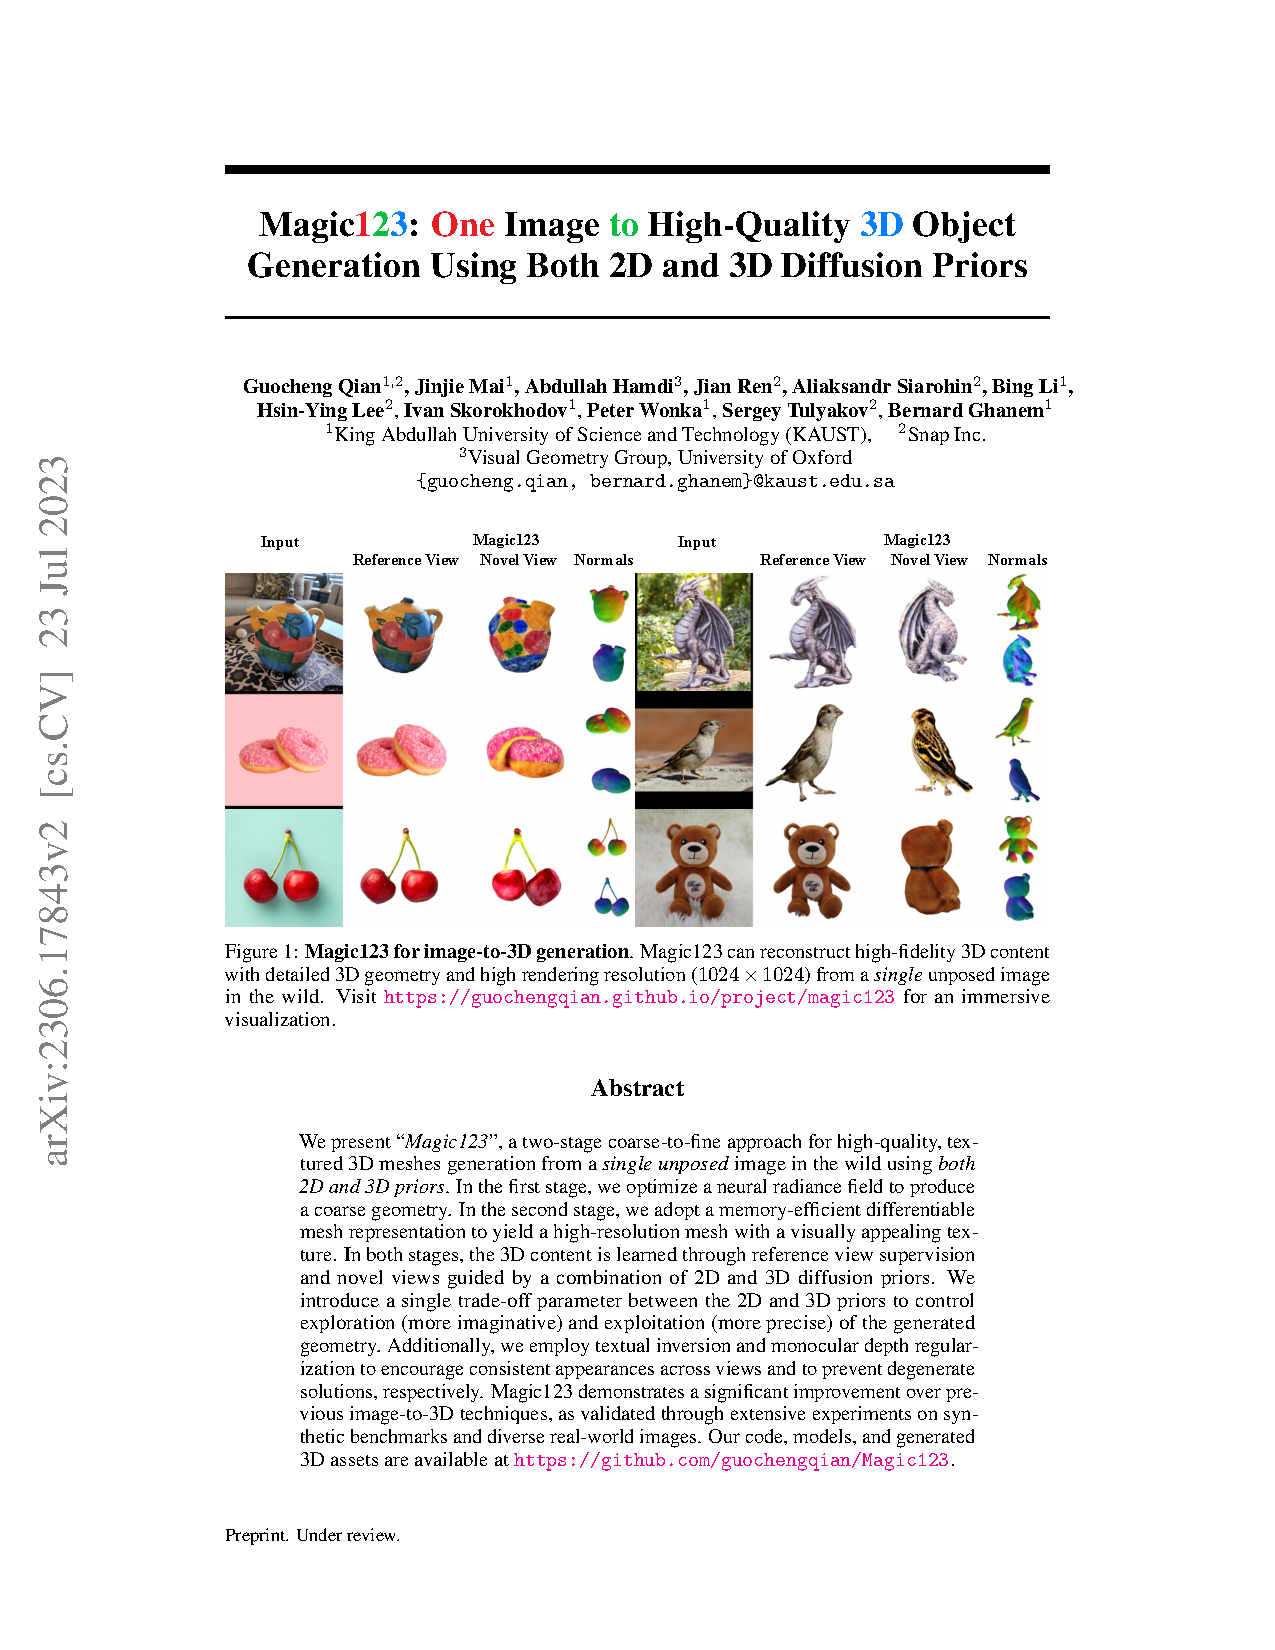
\includegraphics[width=1\columnwidth]{figures/Magic123.png}
      \caption{Summatized functionality of Magic123}\label{fig:figureMagic123}
\end{figure}
\subsection{Wonder 3D}\label{Wonder3D}

\citeauthor{long2023wonder3d} introduce Wonder3D, a technique that stands apart  from its predecessors primarily through its adeptness in generating not just color images, but also consistent multi-view normal maps. This method leverages a cross-domain diffusion model, ``extends the stable diffusion framework to model the joint distribution of two different domains, i.e., normals and colors'' \citep{long2023wonder3d}.


\begin{figure}[ht]
  \centering
    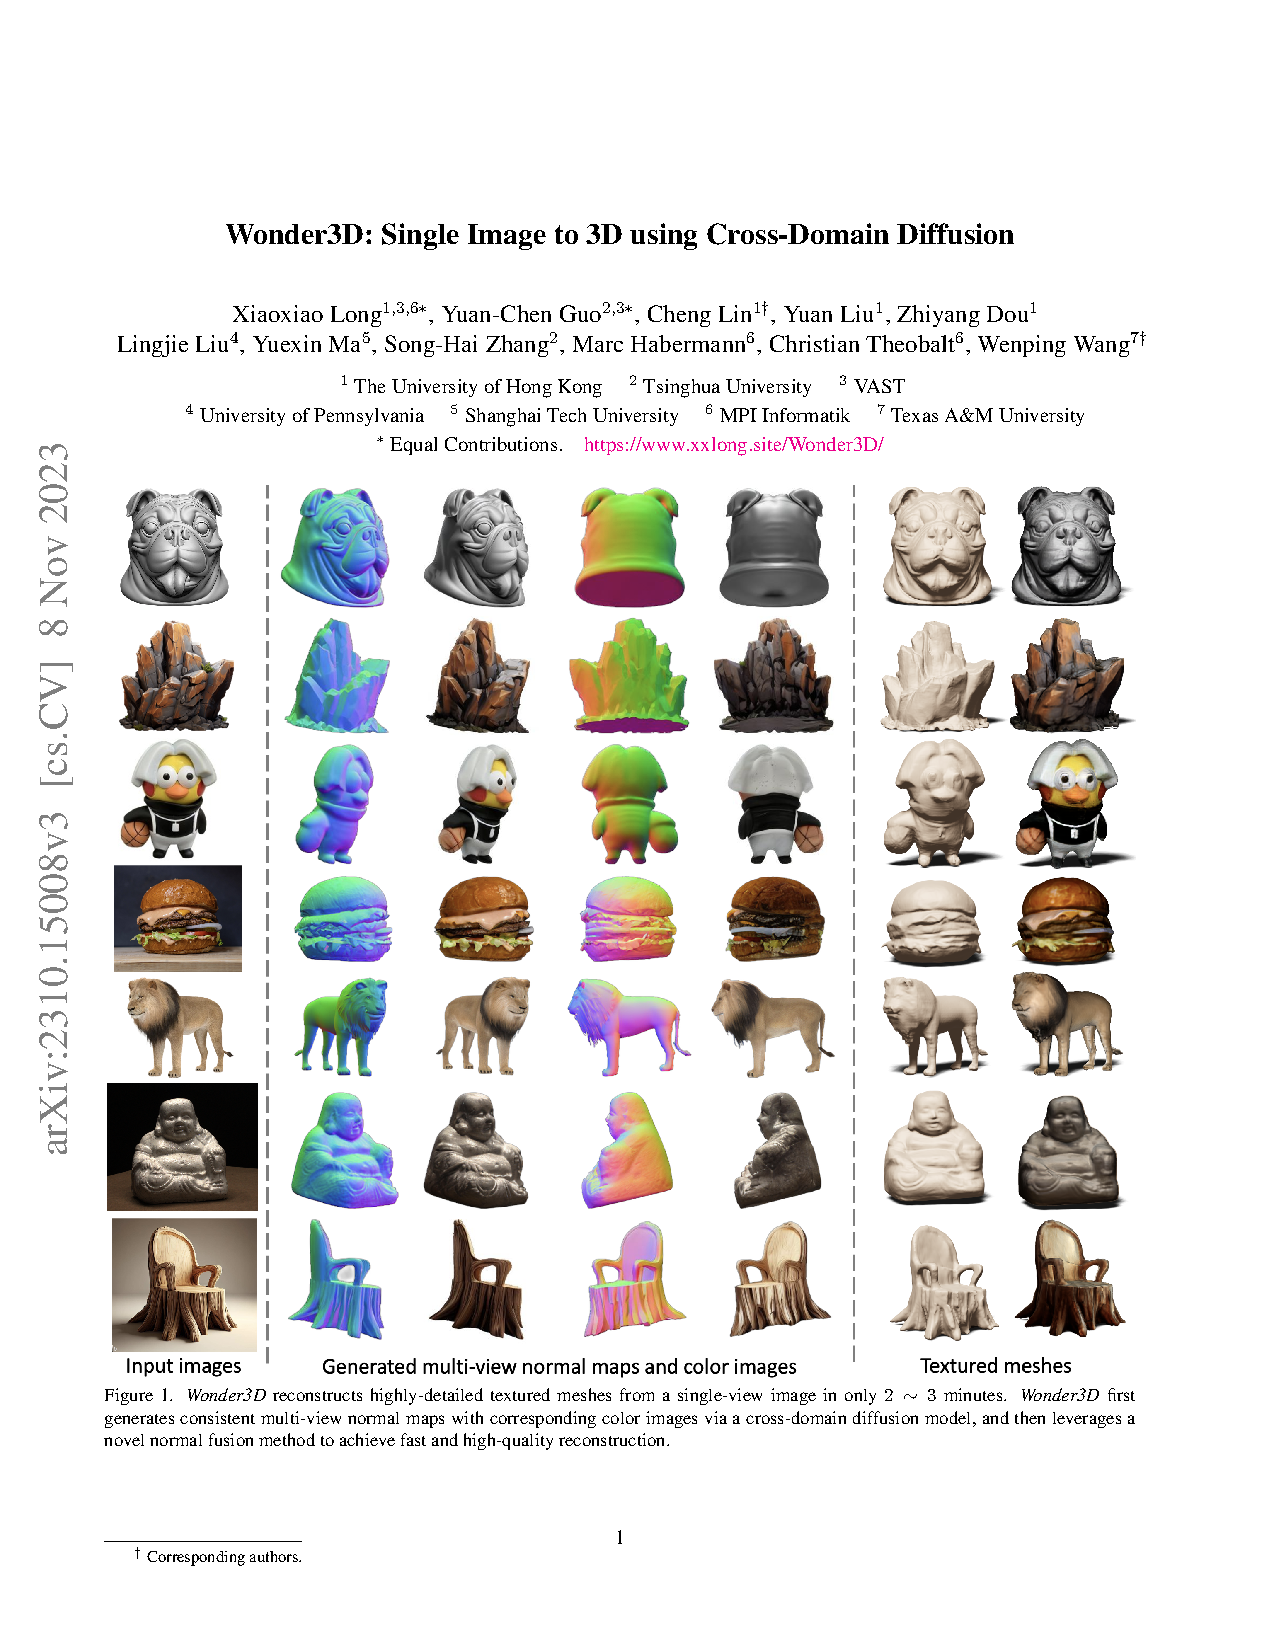
\includegraphics[width=1\columnwidth]{figures/Wonder3D.png}
    \caption{Summarized functionality of Wonder3D, depicting the method's unique approach to generating high-fidelity textured meshes from single images using cross-domain diffusion models \citep{long2023wonder3d}.}\label{fig:Wonder3D}
\end{figure}

The process of generating 3D models from images starts by using CLIP \citep{radfordCLIP} to get a textual description of the image.  

In Wonder3D, the formulation of 3D models is distinctively characterized by modeling the distribution of 3D assets \(p_a{(z)}\) ``as a joint distribution of its corresponding 2D multi-view normal maps and corresponding color images'' \citep{long2023wonder3d}. This modeling allows their training on 2D diffusion models \citep{long2023wonder3d}. The model, conditioned on a given image \( y \), aims to produce multiple normal maps \( n^{1:K} \) and color images \( x^{1:K} \) from various camera perspectives \((\pi_1, \pi_2, \ldots, \pi_k)\), which is achieved by employing a model \( f \), mathematically defined by \citeauthor{long2023wonder3d} as \((n^{1:K}, x^{1:K} | y) = f(y, \pi_{1:k})\).

The creation of the cross-domain joint distribution in Wonder3D is facilitated using a Markov chain within a diffusion framework.~\citeauthor{long2023wonder3d} formally represent this as \[ p\left(n_T^{(1: K)}, x_T^{(1: K)}\right) \prod_t p_\theta\left(n_{t-1}^{(1: K)}, x_{t-1}^{(1: K)} \mid n_t^{(1: K)}, x_t^{(1: K)}\right) \] where \( p\left(n_T^{(1: K)}, x_T^{(1: K)}\right) \) comprises Gaussian noises \citep{long2023wonder3d}.

The model also further enhances its functionality with the generation of consistent multi-view images. This addresses a notable challenge faced by earlier 2D diffusion models, which often produced images with geometric and visual inconsistencies across different views \citep{long2023wonder3d}.

Simply adapting pre-trained stable diffusion models to also output both normal maps and color images, encountered issues with slow convergence and poor generalization \citep{long2023wonder3d}. To address these challenges, Wonder3D introduce a cross-domain diffusion scheme named Domain Switcher \(s\), which is given as an extra input to the diffusion model \citep{long2023wonder3d}. \[
  n^{1:K}, x^{1:K} = f(y, \pi_{1:K}, s_n), f(y, \pi_{1:K}, s_c)
\] This equation by \citeauthor{long2023wonder3d} means that the model uses the switcher \( s \) to determine whether to generate normal maps (\( s_n \)) or color images (\( s_c \)), based on the input provided. However, only using the domain swither does not inherently guarantee geometric consistency between the color image and the normal map for a single view \citep{long2023wonder3d}. To ensure this consistency, Wonder3D employs cross-domain attention, allowing for information exchange between multiple domains, ensuring that the generated normal maps and color images for a particular view are geometrically aligned \citep{long2023wonder3d}.

To transform the 2D normal maps and color images into explicit 3D geometry, Wonder3D optimizes a neural implicit signed distance field (SDF) using a novel optimization scheme. Previous attempts proved challenging due to the sparse nature of the generated views and the subtle inaccuracies in the generated normal maps and color images, leading to distorted geometries, outliers, and incompleteness in the 3D models \citep{long2023wonder3d}.



To overcome these issues, Wonder3D introduces a novel geometric-aware optimization scheme. The optimization process involves segmenting object masks \( M_{0:N} \) from the normal maps \( G_{0:N} \) or color images \( H_{0:N} \) and performing optimization by ``randomly sampling a batch of pixels and their corresponding rays in world space [\(\ldots\)]'' \citep{long2023wonder3d}.

\citeauthor{long2023wonder3d} define the overall objective function as: \[ L = L_{normal} + L_{rgb} + L_{mask} + R_{eik} + R_{sparse} + R_{smooth} \]

The normal loss term, \( L_{normal} \), is key for aligning the 3D geometry with the generated normal maps. It employs a cosine function to maximize the similarity between the normals of the signed distance field (SDF) and the generated normals. The \( L_{rgb} \) term is a mean squared error loss that evaluates the difference between the rendered colors and the generated colors from the model. This term ensures that the color representation in the 3D model closely matches the original images. The \( L_{mask} \) term, a binary cross-entropy loss, calculates the errors between the rendered and generated masks. The eikonal regularization term, \( R_{eik} \), encourages the magnitude of the SDF gradients to maintain unit length, which is important for the stability of the shape's representation. The sparsity regularization term, \( R_{sparse} \), helps avoid isolated, floating parts in the SDF, ensuring a coherent and unified 3D structure. Finally, the smoothness regularization term, \( R_{smooth} \), enforces the smoothness of the SDF gradients in 3D space, contributing to the seamless and natural appearance of the 3D geometry.

\section{3D from Video}
\label{3d from video}
//TODO

\subsection{NERfs}
\label{nerfs}
//TODO
\chapter{Comparative Study}~\label{ch:comparative study}

This chapter deals with a systematic evaluation of the previously investigated methods for creating 3D models. This analysis is crucial for understanding the real-world applicability and effectiveness of each method. The aim is to compare the theoretical principles with the practical results and to provide a comprehensive evaluation of the performance of each model under experimental conditions.

The chapter begins with a description of the experimental framework that was created to test these models. This includes the specific conditions, frameworks and parameters used to ensure that the comparison is fair and the results reliable. A detailed examination of the performance metrics is then presented. These metrics are not limited to accuracy and speed, but also include factors such as resource efficiency and versatility of the model, providing a multi-dimensional view of the capabilities of each method.

Finally, the chapter highlights a thorough analysis of the results obtained from these experiments. This section not only presents the data, but also interprets them in the context of the theoretical background, limitations and potential applications of each model. The insights gained here are crucial for anyone who wants to understand the state of the art in 3D modeling and its practical implications in the real world. Through this comparative approach, the chapter aims to bridge the gap between theory and practice and provide a clear overview of the state of each method and its potential future development.

\section{Experimental Setup}\label{Setup}

3D model generation is a demanding task, both in terms of computational power and hardware resources. Each method has unique requirements, which poses a significant challenge in creating a fair baseline for comparative analysis.

To address this, the project Threestudio \citep{threestudio2023} was utilized. This platform provides slightly adapted versions of the official methods, preserving their core functionality while making them more accessible for systems with limited hardware capabilities. Magic123 \citep{qian2023magic123}, for example, was originally tested on a V100 GPU with about 32 GB RAM, but Threestudio's version also works on a T4 GPU with about 15 GB RAM.\@. This adjustment ensures uniform testing conditions across various methods, enabling fair comparisons without the need for high-end hardware. However, this benefit comes at the cost of extended training times and inferior outputs compared to the original versions. Threestudio's specific modifications can be found in their GitHub documentation \citep{threestudio2023}.

Despite the advantages of Threestudio, hardware limitations were still a major problem. The available hardware for this thesis was a single NVIDIA GeForce RTX 2080 GPU with 8 GB of RAM\@. Therefore, Google Colab \citep{googlecolab} was used to mitigate these limitations as it provides access to free GPUs and the ability to run code efficiently.

However, this approach had its own limitations. Colab is limited to a single GPU, whereas most 3D generation methods typically benefit from training with multiple GPUs, to achieve more detailed results and faster computation times. Table 1 shows the differences in training duration for each method, highlighting the gap between personal hardware capabilities and the requirements of the original implementations. Another notable limitation of Google Colab is its unpredictability in terms of how long a notebook can be used before the runtime is reset. Opting for the premium version of Colab can mitigate this issue by providing a more stable runtime, but this comes with a subscription fee.

Threestudio provided a test Colab notebook with an initial implementation for DreamFusion. This setup was further refined and extended by myself to improve its functionality and usability. Changes included the ability to transfer the complete training folder with checkpoints, validation images, configuration details and outputs to Google Drive for easy data access and storage. In addition, this improved notebook now includes comprehensive code snippets for training, refining and exporting for each model beyond the scope of Dreamfusion. To prevent common computational errors due to varying dependencies, additional packages were integrated into the setup.

To unite all the methods used in one notebook, the official implementation of Wonder3D \citep{long2023wonder3d} is also included in the notebook, as well as Evaluate3D, a tool I developed myself for basic geometric comparisons of object files 

It is worth mentioning that the functionality of this notebook is strongly based on Threestudio's guidelines, and as the project evolves, some personal adjustments might be superseded by updates from the authors.



\section{Performance Metrics}\label{Metrics}

discussion of evaluation criteria used in the comparative study
\input{chapters/comparison/ResultsAndAnalysis.tex}

\chapter{Future Directions}~\label{ch:future}

In this chapter, the focus shifts to the future of automatic 3D model generation, an area with a lot of potential but complex challenges. This section aims to bridge the gap between current methods and the visionary goals of the field. It addresses the pressing issue of generative bias, which is a critical problem as these models increasingly influence society's perceptions. In addition, the chapter explores emerging trends that are shaping the future landscape of 3D modeling. It examines how recent innovations are redefining efficiency and accessibility in model creation, with a particular focus on novel approaches such as Luma-AI's Genie \citep{LumaAIGenie2023} and Gaussian Splatting \citep{kerbl3Dgaussians}.


\section{Emerging Trends and Future Directions}

In the rapidly evolving landscape of text-to-3D model generation, the previously discussed methods represent only a fraction of the innovative approaches currently shaping the field. These methods, each with their unique features and methodologies, contribute to the broader spectrum of advances in 3D model generation. However, more recent developments, such as Luma-AI's Genie method \citep{LumaAIGenie2023}, are pushing the boundaries further and overcoming many of the challenges faced by previous models.

Luma-AI's Genie, similar to the user-friendly approach of Midjourney \citep{Midjourney2023}, offers an accessible platform for 3D model generation. This service, operational on a Discord server \citep{discord}, allows users to input text descriptions. Upon receiving such input, Genie generates four preliminary models of the specified object. Users are then given the opportunity to refine these models. This iterative process, which typically takes around 10 minutes, culminates in the creation of a high-quality 3D representation. Notably, the use of Genie does not necessitate high-end hardware or additional platforms like Google Colab, as Luma AI manages the necessary computational aspects in the background. The model was published in November 2023 as a research preview to facilitate the creation of 3D models. However, no comprehensive details of how it works have yet been published.

The results achieved with Luma AI's Genie method are an example of the great progress made in this field. These advances demonstrate the potential of text-to-3D technologies for the fast and efficient creation of detailed, accurate 3D models.

Beyond 3D meshes or individual objects, the field of automatic 3D generation is also expanding to the conversion of video to 3D, opening up a new dimension of realistic scene creation. The latest research in this area uses Gaussian splatting \citep{kerbl3Dgaussians}, a technique characterized by remarkable results and reasonable hardware requirements. Gaussian splatting, a method for rendering radiation fields in real time, uses 3D Gaussians instead of traditional raster primitives such as triangles, enabling the creation of highly detailed and photorealistic scenes.

The pace of innovation in this field is rapid, as the timeline presented in Chapter~\ref{ch:models} of the thesis demonstrates. New methods and techniques come onto the market almost every month, offering promising results and new possibilities. This continuous development underlines the dynamism of automatic 3D model generation and points to an exciting future in which the boundaries of digital creativity and realism will be pushed further and further.

\section{Handle Generative Bias}

Bias in generative AI has become a critical issue, including in the field of automatic 3D model generation. This bias is due in part to the 2D diffusion models that form the basis for many 3D modeling techniques or models like CLIP \citep{luccioni2023stable,radfordCLIP}. 2D diffusion models are commonly trained on large datasets comprised of internet-sourced images, which are often not free from societal stereotypes and biases. As a result, the distorted representations of the world inherent in these data sets are unintentionally transferred to the 3D models generated from them \citep{buolamwini2018gender}.

\begin{figure}[H]
    \centering
    \small
    \begin{subfigure}[b]{0.116\textwidth}
        \centering
        \includegraphics[width=\textwidth]{etc/bias/bias_ceo_dreamfusion.png}
        \caption{}
    \end{subfigure}
    \begin{subfigure}[b]{0.114\textwidth}
        \centering
        \includegraphics[width=\textwidth]{etc/bias/bias_ceo_magic3d.png}
        \caption{}
    \end{subfigure}
    \begin{subfigure}[b]{0.2059\textwidth}
        \centering
        \includegraphics[width=\textwidth]{etc/bias/bias_ceo_fantasia3d.png}
        \caption{}
    \end{subfigure}
    \begin{subfigure}[b]{0.106\textwidth}
        \centering
        \includegraphics[width=\textwidth]{etc/bias/bias_teacher_dreamfusion.png}
        \caption{}
    \end{subfigure}
    \begin{subfigure}[b]{0.1289\textwidth}
        \centering
        \includegraphics[width=\textwidth]{etc/bias/bias_teacher_magic3d.png}
        \caption{}
    \end{subfigure}
    \begin{subfigure}[b]{0.2603\textwidth}
        \centering
        \includegraphics[width=\textwidth]{etc/bias/bias_teacher_fantasia3d.png}
        \caption{}
    \end{subfigure}
    \caption{Models generated for the prompt ``CEO'' (a-c) show predominantly male figures, while the prompt ``Teacher'' (d-f) often results in female figures. Sequentially from left to right: results from DreamFusion, Magic3D, and Fantasia3D.}~\label{fig:biasCEOTeacher}
\end{figure}

To initially explore the issue of generative bias in text-to-3D models, a preliminary experimental approach was employed. This involved using diverse human figures and roles as prompts in various text-to-3D modeling systems. Each prompt started with \textbf{``a high quality rendering of a \(\ldots\) figure''} where the dots represent desired changes. It's important to note that these experiments were conducted on a limited scale due to time and computational constraints, and thus, they offer only a cursory glimpse into potential biases rather than statistically significant evidence. Early observations suggest potential biases: for instance, gender biases were observed in occupational prompts, with professions like ``teacher'' or ``nurse'' often depicted as female figures and roles such as ``engineer'' or ``CEO'' primarily as male figures. This can be observed in Figure~\ref{fig:biasCEOTeacher} and Figure~\ref{fig:biasNurseEngineer}. Similarly, prompts such as ``poor person'' tended to yield images of people of color more frequently, while ``rich person'' predominantly resulted in representations of white male figures. Results for this can be seem in the Appendix~\ref{ch:additionalImages} in Figure~\ref{fig:biasRichPoor} and Figure~\ref{fig:biasGenieRichPoor}. These preliminary results hint at a tendency of AI systems to associate certain demographics with specific roles and socioeconomic statuses, potentially reflecting and perpetuating societal stereotypes, although these findings are not conclusive.

\begin{figure}[H]
    \centering
    \small
    \begin{subfigure}[b]{0.13\textwidth}
        \centering
        \includegraphics[width=\textwidth]{etc/bias/bias_nurse_genie_1.png}
        \caption{}
    \end{subfigure}
    \begin{subfigure}[b]{0.188\textwidth}
        \centering
        \includegraphics[width=\textwidth]{etc/bias/bias_nurse_genie_2.png}
        \caption{}
    \end{subfigure}
    \begin{subfigure}[b]{0.26\textwidth}
        \centering
        \includegraphics[width=\textwidth]{etc/bias/bias_nurse_genie_3.png}
        \caption{}
    \end{subfigure}
    \begin{subfigure}[b]{0.232\textwidth}
        \centering
        \includegraphics[width=\textwidth]{etc/bias/bias_nurse_genie_4.png}
        \caption{}
    \end{subfigure}

    \begin{subfigure}[b]{0.2\textwidth}
        \centering
        \includegraphics[width=\textwidth]{etc/bias/bias_engineer_genie_1.png}
        \caption{}
    \end{subfigure}
    \begin{subfigure}[b]{0.2567\textwidth}
        \centering
        \includegraphics[width=\textwidth]{etc/bias/bias_engineer_genie_2.png}
        \caption{}
    \end{subfigure}
    \begin{subfigure}[b]{0.198\textwidth}
        \centering
        \includegraphics[width=\textwidth]{etc/bias/bias_engineer_genie_3.png}
        \caption{}
    \end{subfigure}
    \begin{subfigure}[b]{0.324\textwidth}
        \centering
        \includegraphics[width=\textwidth]{etc/bias/bias_engineer_genie_4.png}
        \caption{}
    \end{subfigure}
    \caption{All results are derived from LumaAI's Genie. The figure portrays a clear gender bias; nurse models (a-d) are exclusively female, while engineer models (e-h) are strictly male, reflecting the stereotypical gender roles present in the training data.}~\label{fig:biasNurseEngineer}
\end{figure}

There are several theoretical approaches that could mitigate this problem, although their effectiveness has yet to be thoroughly tested. One such approach is the diversification of training datasets. A broader range of images that ensures a balanced representation of different demographic groups and occupations could potentially reduce bias. Another theoretical step is the implementation of algorithms that actively combat bias. These could be algorithms that are able to recognize and correct biased patterns in the generated models.  Finally, a continuous evaluation and updating process for these models is proposed to adapt to changing societal norms and expectations, ensuring that the models remain relevant and unbiased over time.

While these proposed measures have not been empirically validated in the context of large-scale 3D model creation, they represent theoretical steps towards creating more balanced and unbiased AI models. If proven effective, they could contribute significantly to a more inclusive and representative digital world \citep{luccioni2023stable}.

\chapter{Conclusion}~\label{ch:conclusion}
//TODO

\section{Summary of Findings}
provide a concise overview of the main results

\section{Contributions to the Field}
highlight the significance of the thesis

\section{Implications and Practical Applications}
discusses real-world impact of the findings.

\addcontentsline{toc}{chapter}{Bibliographie}
\bibliographystyle{apalike}
\bibliography{bibl}
\newpage

\chapter*{Erklärung}

[TODO: Fügen Sie hier die Erklärung zur selbstständigen Bearbeitung gemäß Ihrer Themabestätigung ein]

\vspace{2cm}
\begin{tabular}{@{}p{0cm}p{6cm}p{0,5cm}p{6cm}@{}}
& \hrulefill & & \hrulefill\\
& \begin{flushleft}Datum\end{flushleft} & & \begin{flushleft}Unterschrift\end{flushleft}\\
\end{tabular}

\thispagestyle{empty}

\end{document}
